\section{Introduction}

While techniques for analysing the dependency structure of programs have been very fruitful, with applications ranging from information-flow security~\cite{sabelfeld03} and optimisation~\cite{kildall73} to debugging and program comprehension~\cite{weiser81,delucia96}, methods suitable for analysing richly structured outputs such as data visualisations and matrices are less common. Where-provenance~\cite{buneman01} and related data provenance techniques are fine-grained but are usually restricted to relational query languages. Taint tracking \cite{newsome05} tends to be low-level approach and restricted to tracking taint forwards from input to output. Dataflow analyses \cite{reps95} focus on analysing variables rather than parts of structured values.

For programs which transform richly structured inputs into richly structured outputs, such as visualisation code which turns tables of data into charts, or array computations which operate on large multidimensional structures, we need analysis tools that let us focus on a particular part of the output, so that we can isolate the input dependencies pertinent only to that part of the output. Recent program slicing techniques \cite{perera12a,perera13a,ricciotti17} allow the user to focus on the output by ``erasing'' parts deemed to be irrelevant; the erased parts, called \emph{holes}, are propagated backwards by a backwards analysis which identifies parts of the program and input which are no longer needed. Although these approaches enjoy useful round-tripping properties characterised by Galois connections, they only allow focusing on \emph{prefixes} of a structured output, rather than arbitrary substructures.

These problems are no longer just relevant to programmers. Every day, journalists and scientists curate data into charts and other visual summaries which must be interpreted by colleagues, policy makers and lay readers alike. But charts can be hard to interpret correctly, even with access to the source code and data sets. Innocent (but devastating) mistakes such as transposing two columns of data have gone unnoticed for several years, even in widely cited papers~\cite{miller06}. Less innocent mistakes are deployed by politicians to mislead voters~\cite{fullfact19}. For the sake of transparency and trust, it is vital that content consumers, as well as content creators, are able to easily verify for themselves how visual outputs relate to the data they are derived from.

Understanding and trusting a visualisation, even for an expert, means knowing what its visual attributes actually \emph{represent}, which in turn involves the following two comprehension challenges:

\begin{enumerate}
  \item understanding the mapping between the data source and visual elements;
  \item understanding how different views of the same data are related.
\end{enumerate}

\subsection{Fine-grained linking between outputs and inputs}

\noindent From a program analysis perspective, each of these presents an interesting problem. For (1), we want to be able to focus on a visual element and see what inputs contribute to it. This is a matter of selecting a part of the structured output and performing a backwards analysis that identifies parts of the input data and perhaps parts of the program that contribute to the selected output. This is illustrated on the left-hand side of \figref{introduction:vis-linking} below:

\begin{figure}[H]
   {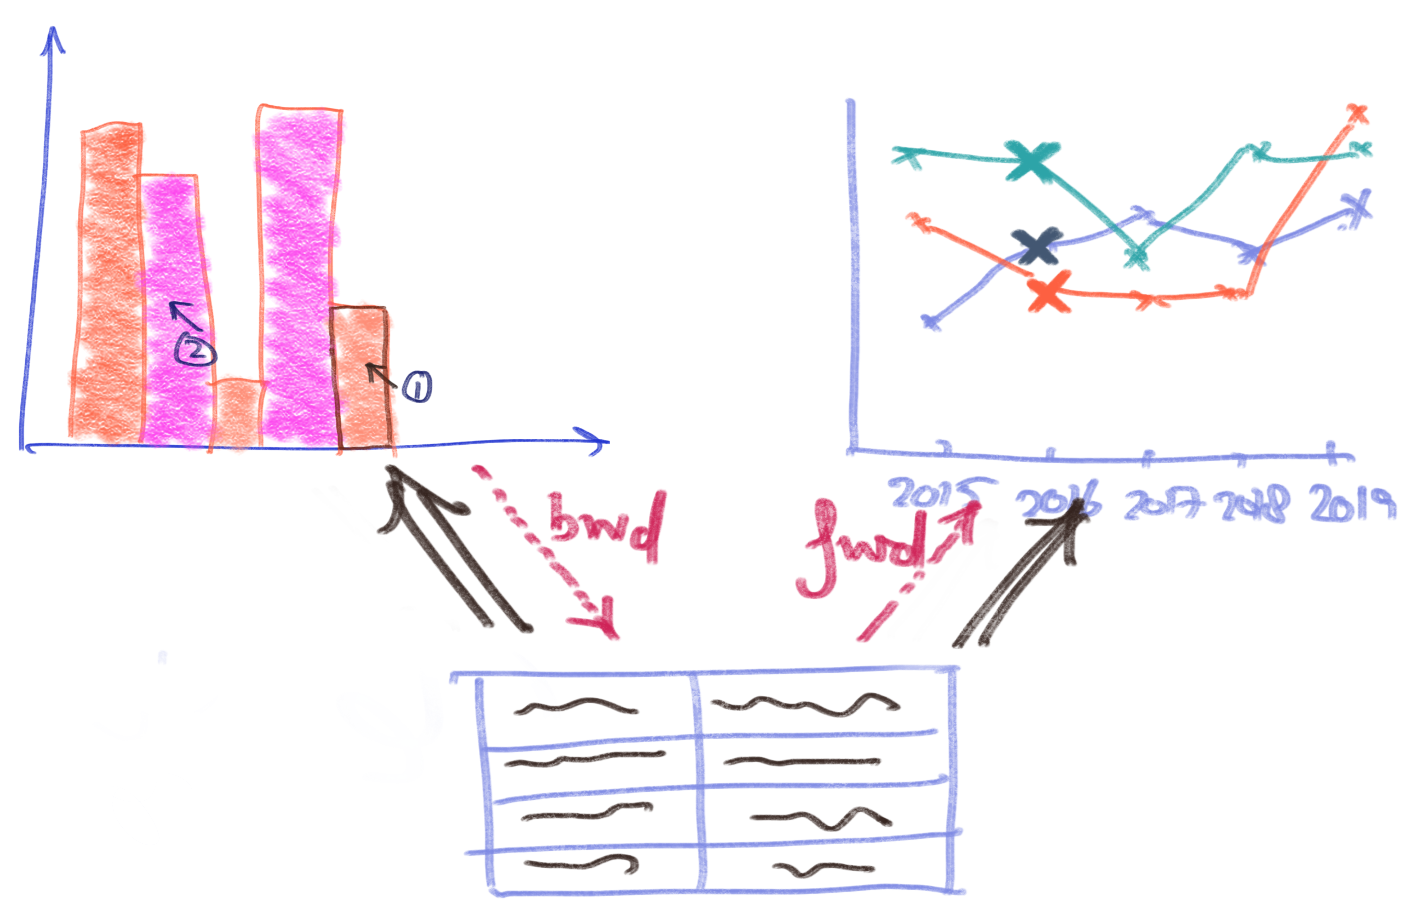
\includegraphics[scale=0.14]{fig/example/vis-linking.png}}
   \small
   \begin{lstlisting}
      let data = [ ... ]
      let barchart = data |> some transformation
      let linechart = data |> some other transformation
   \end{lstlisting}
   \caption{Linking cognate visualisations via common data dependencies}
   \label{fig:introduction:vis-linking}
\end{figure}

Visualisation designers do sometimes create ``data-linked'' artefacts like these by hand, such as Nadieh Bremer's award-winning visualisation of population density growth in Asian cities~\cite{bremer15}. But crafting such things by hand is a significant undertaking, requiring intimate knowledge of the computational relationship between chart and data, and programming effort to expose that information to the reader. Manual approaches are also error-prone and needs to be changed whenever the application logic changes. A library-based approach would improve on this, but would only provide data linking for solutions that can be readily expressed using the library. By framing this as a program analysis problem, visualisation code can be completely oblivious to these additional transparency features. The data scientist or visualisation designer need concern themselves only with constructing the appropriate view as a function of the data, leaving the programming language to take care of linking the outputs to the data sources in a fine-grained way.

\subsection{Fine-grained linking between distinct outputs}

Problem (2) is more challenging; we want to be able to focus on a visual element in one chart or graphic and see what aspects of a different chart are computed using related inputs. This is a matter of again selecting a part of the structured output and performing a backwards analysis to identify the required inputs, but then performing a further forwards analysis to identify dependent parts of the other output. The forward analysis part is shown on the right-hand side of \figref{introduction:vis-linking} above.

[ORIGINAL VERSION]

To address this, much work in data visualization has been done to assist analysts understand the mapping between data source and visual elements in the visualization and understand how different views of the same data are related. This is typically done through data visualization lirbaries that do not utilize rich program analysis techniques.

\section{Introduction}

\noindent Even with the data and source code used to create the visualisation to hand, answering questions such as these is difficult, requiring time and expertise. The basic problem is that visualisations are opaque, disconnected from the data and computations used to create them. This situation would be significantly imporved if visualisations allowed a reader to explore the relationship to the underlying data through the visualisation itself, revealing the relevant connections on a need-to-know basis, as the reader interacts with it (see left-hand side of \figref{introduction:viz-linking} below):

Given that a visualisation is a view computed from a data source, it seems plausible that we might adapt techniques from program analysis and data provenance to provide a runtime infrastructure that automatically supports linked selections.

\subsection{Linking visualisations to each other}

It is also common to use more than one view to present distinct but related aspects of data. (We say visualisations are \emph{cognate} when they are related in this way.) Geospatial applications like GeoDa~\cite{anselin06} and charting libraries like Plotly provide a view coordination feature called \emph{brushing and linking}~\cite{becker87}, where selections in one chart automatically select corresponding elements in the other, as an aid to comprehension. In \figref{introduction:vis-linking} below, selecting a bar on the left automatically selects all the related visual elements on the right. Although such coordination features are highly desirable, they are either baked into specific applications, or require programmer effort and therefore must be anticipated in advance by the chart designer. Moreover the linking is opaque, providing no direct way for the reader to see the data which underpins the relationship.

\subsection{Our contributions}

In this paper, we present new language-based data provenance techniques for linking visualisations to data, and to each other, in a fine-grained way. Our specific contributions are as follows:

\begin{itemize}[leftmargin=*]
   \item[--] a review of \emph{Galois slicing}, a program slicing framework with round-tripping properties appropriate to our problem, and an analysis of its shortcomings (\secref{background});
   \item[--] a new bidirectional dependency analysis inspired by Galois slicing, addressing these shortcomings, for a core calculus with lists and arrays, and a discussion of how the components of this analysis can be combined in various ways to link inputs to outputs and outputs to other outputs (\secref{core-language});
   \item[--] a richer surface language called \OurLanguage with familiar functional programming features, including piecewise definitions, pattern matching, list notation and list comprehensions, and an extension of our analysis to the desugaring (\secref{surface-language});
   \item[--] an implementation of Fluid in PureScript, and a discussion and evaluation of the strengths and weaknesses of our approach (\secref{implementation}).
\end{itemize}
